\documentclass{standalone}

\usepackage{tikz}

\usetikzlibrary{arrows}
\usetikzlibrary{decorations.markings}

\begin{document}
  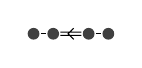
\begin{tikzpicture}
    \pgfdeclaredecoration{zdouble}{initial}{
      \state{initial}[width=\pgfdecoratedinputsegmentlength]{
        \pgfmathsetlengthmacro\lw{\pgflinewidth+.5\pgflinewidth}
        \pgfmathsetlengthmacro\lma{ 1.0pt+.5*\pgfdecoratedinputsegmentlength}
        \pgfmathsetlengthmacro\lmb{-1.0pt+.5*\pgfdecoratedinputsegmentlength}
        \begin{pgfscope}
          \pgfpathmoveto{\pgfpoint{0pt}{\lw}}%
          \pgfpathlineto{\pgfpoint{\pgfdecoratedinputsegmentlength}{ \lw}}%
          \pgfpathmoveto{\pgfpoint{0pt}{-\lw}}%
          \pgfpathlineto{\pgfpoint{\pgfdecoratedinputsegmentlength}{-\lw}}%
          \pgfmoveto{\pgfpoint{\lmb}{ 2.0pt}}%
          \pgfpathlineto{\pgfpoint{\lma}{0pt}}%
          \pgfpathlineto{\pgfpoint{\lmb}{-2.0pt}}%
        \end{pgfscope}
      }
    }
    \tikzstyle{vn} = [color=darkgray          , circle, outer sep=0.5pt, fill, inner sep=1.5pt]
    \tikzstyle{ed} = [decorate,decoration={zdouble}]

    \node[vn] (1) at ( 0.00, 0.00) {};
    \node[vn] (2) at ( 0.25, 0.00) {};
    \node[vn] (3) at ( 0.70, 0.00) {};
    \node[vn] (4) at ( 0.95, 0.00) {};
    \draw (1) -- (2);
    \draw[ed] (3) -- (2);
    \draw (3) -- (4);
  \end{tikzpicture}
\end{document}
